%%%%%%%%%%%%%%%%%%%%%%%%%%%%%%%%%%%%%%%%%%%%%%%%%%%%%%%%%%%%%%%%%%%%%%%%%%%%%%%%%%%%%%%%%%%%%%%%%%%%%%%%%%%%%%%%%%%%%%%%%%%%%%%%%%%%%%%%%%%%%%%%%%%%%%%%%%%
% This is just an example/guide for you to refer to when submitting manuscripts to Frontiers, it is not mandatory to use Frontiers .cls files nor frontiers.tex  %
% This will only generate the Manuscript, the final article will be typeset by Frontiers after acceptance.   
%                                              %
%                                                                                                                                                         %
% When submitting your files, remember to upload this *tex file, the pdf generated with it, the *bib file (if bibliography is not within the *tex) and all the figures.
%%%%%%%%%%%%%%%%%%%%%%%%%%%%%%%%%%%%%%%%%%%%%%%%%%%%%%%%%%%%%%%%%%%%%%%%%%%%%%%%%%%%%%%%%%%%%%%%%%%%%%%%%%%%%%%%%%%%%%%%%%%%%%%%%%%%%%%%%%%%%%%%%%%%%%%%%%%

%%% Version 3.4 Generated 2018/06/15 %%%
%%% You will need to have the following packages installed: datetime, fmtcount, etoolbox, fcprefix, which are normally inlcuded in WinEdt. %%%
%%% In http://www.ctan.org/ you can find the packages and how to install them, if necessary. %%%
%%%  NB logo1.jpg is required in the path in order to correctly compile front page header %%%

\documentclass[utf8]{frontiersSCNS} % for Science, Engineering and Humanities and Social Sciences articles
%\documentclass[utf8]{frontiersHLTH} % for Health articles
%\documentclass[utf8]{frontiersFPHY} % for Physics and Applied Mathematics and Statistics articles

%\setcitestyle{square} % for Physics and Applied Mathematics and Statistics articles
\usepackage{url,hyperref,lineno,microtype,subcaption}
\usepackage[onehalfspacing]{setspace}
\epstopdfsetup{outdir=./}

\linenumbers


% Leave a blank line between paragraphs instead of using \\


\def\keyFont{\fontsize{8}{11}\helveticabold }
\def\firstAuthorLast{Mrad {et~al.}} %use et al only if is more than 1 author
\def\Authors{Assaad Mrad\,$^{1,*}$, Mazen Nakad\,$^{1}$, Yanlan Liu\,$^{1}$ Jean-Christophe Domec\,$^{1,2}$, Sanna Sevanto\,$^{3}$ and Gabriel Katul\,$^{1,4}$}
% Affiliations should be keyed to the author's name with superscript numbers and be listed as follows: Laboratory, Institute, Department, Organization, City, State abbreviation (USA, Canada, Australia), and Country (without detailed address information such as city zip codes or street names).
% If one of the authors has a change of address, list the new address below the correspondence details using a superscript symbol and use the same symbol to indicate the author in the author list.
\def\Address{$^{1}$Nicholas School of the Environment, Duke University, Durham, NC, USA \\
$^{2}$ UMR INRA-ISPA 1391, Bordeaux Sciences Agro, Gradignan 33195, France \\
$^{3}$Earth and Environmental Sciences Division, Los Alamos National Laboratory, Los Alamos, New Mexico, USA \\
$^{4}$Department of Civil and Environmental Engineering, Duke University, Durham, NC}
% The Corresponding Author should be marked with an asterisk
% Provide the exact contact address (this time including street name and city zip code) and email of the corresponding author
\def\corrAuthor{Assaad Mrad}

\def\corrEmail{mradassaad2@gmail.com}




\begin{document}
\onecolumn
\firstpage{1}

\title[Dynamic optimality principle for water use strategies]{A dynamic optimality principle for water use strategies explains isohydric to anisohydric plant responses} 

\author[\firstAuthorLast ]{\Authors} %This field will be automatically populated
\address{} %This field will be automatically populated
\correspondance{} %This field will be automatically populated

\extraAuth{}% If there are more than 1 corresponding author, comment this line and uncomment the next one.
%\extraAuth{corresponding Author2 \\ Laboratory X2, Institute X2, Department X2, Organization X2, Street X2, City X2 , State XX2 (only USA, Canada and Australia), Zip Code2, X2 Country X2, email2@uni2.edu}


\maketitle


\begin{abstract}

%%% Leave the Abstract empty if your article does not require one, please see the Summary Table for full details.
\section{}
For full guidelines regarding your manuscript please refer to \href{http://www.frontiersin.org/about/AuthorGuidelines}{Author Guidelines}.

As a primary goal, the abstract should render the general significance and conceptual advance of the work clearly accessible to a broad readership. References should not be cited in the abstract. Leave the Abstract empty if your article does not require one, please see \href{http://www.frontiersin.org/about/AuthorGuidelines#SummaryTable}{Summary Table} for details according to article type. 


\tiny
 \keyFont{ \section{Keywords:} keyword, keyword, keyword, keyword, keyword, keyword, keyword, keyword} %All article types: you may provide up to 8 keywords; at least 5 are mandatory.
\end{abstract}

\section{Introduction}

Gas exchange at the level of the stomata supports all plant life on earth by providing energy in the form of carbon dioxide ($CO_2$) for growth and maintenance in exchange for water. Over the past millenia, as atmospheric $CO_2$ concentrations decreased ten-fold and an increasing number of plant species adapting to terrestrial ecosystems, the need to optimize carbon gain in relation to water loss arose. This is thought to be behind the adaptation of cacti to arid climates by using a different photosynthetic machinery denoted as Crassulacean Acid Metabolism (CAM) photosynthesis. CAM photosynthesis allows stomata to open at night, when temperature and the vapor pressure deficit (VPD) are low so as to minimize loss of water. It is thought that the stomatal opening of plants utilizing C3 and C4 photosynthesis is also governed by water limitations.

In fact, multiple models grounded on stomatal optimization were put forward and tipped as accurate predictors of transpiration. The accuracy those predictions is crucial for climate forecasting. \textbf{Here offer summary of these models}.

While the assumption that stomatal opening trends are controlled by plant hydraulics is widely used in the plant community, there is a shortage of evidence corroborating this assumption. In this work, the effect of plant water use strategies (from conservative to aggressive) on stomatal conductance ($g$) and leaf water potential ($\psi_l$) is analyzed through a dynamical system perspective that allows setting multiple constraints. 

\citet{Manzoni2013} offer a similar dynamical system approach to the same phenomenon. Water use strategy is prescribed by assigning a 'carbon value' to the terminal soil moisture content around the rooting zone. This study is similarly framed with additional sub-daily measured forcings and constraints on water use such as neighboring tree competition. The results of this model are compared to actual measurements.

The work here answers the following question: to what degree does water use strategy dictate stomatal control during dry-down? In a recent review of the theory of optimal stomatal control, \citet{Buckley2017} recognize the importance of delayed benefits such as keeping soil soil moisture at higher levels for future use. 

The goal here is not to develop a stomatal prediction package but to explore whether plant hydraulic traits alone are capable of placing stomatal behavior anywhere on the iso- or aniso-hydry spectrum. 

\section{Materials and Methods}

\subsection{Theory}

The principle adopted here is that plants maximize their carbon gain ($A$) over the period of a drydown. This principle assumes that plants freely control the stomatal conductance $g_s$. Previous work constrained control of $g_s$ by enforcing instantaneous water balance at the soil level \citep{Manzoni2013}. To mathematically express this constraint an augmented Lagrangian is defined $H$:
\begin{equation}
    \label{eqn:Hamiltonian}
    H\Big(g_s, x, \frac{dx}{dt}, \lambda, t\Big) = A(g_s, t) + \lambda f_e\Big(g_s, x, \frac{dx}{dt}, t\Big).
\end{equation}
$\lambda$ is the Lagrange multiplier, $x$ is the soil moisture, $t$ is time, and $f_e$ is the soil water balance.

Because the principle states that $A$ is maximized over a drydown, the objective function $J$ is the integral of $H$ from $t=0$ at the beginning of drydown to $t=T$ at the end of it:
\begin{equation}
    \label{eqn:Objective}
    J\Big(g_s, x, \frac{dx}{dt}, \lambda, t\Big) = \int_0^T H\Big(g_s, x, \frac{dx}{dt}, \lambda, t\Big).
\end{equation}

The goal then consists of finding the function of $g_s$ in terms of $t$ that maximizes $J$. This goal is achieved by solving the Euler-Lagrange equations using the method of the calculus of variations. A required step however is expressing $A$ and $f_e$ in terms of the control variable $g_s$ and the state variable $x$.

\subsection{Carbon gain}

The seminal work by \citet{Farquhar1980} expresses carbon assimilation, or biochemical demand of carbon $A_{demand}$, for a C3 leaf as either limited by the Rubisco enzyme activity under saturated incoming photosynthetically active radiation (PAR) or by ribulose-1,5-biphosphate (RuBP) activity under limiting incoming PAR. 
To avoid the use of non-linear functions such as the minimum between two number as well as ad-hoc parameters that might remedy this non-linearity, we adopt an accurate approximation to $A_{demand}$ \citep{Vico2013}. $A_{demand}$ is approximated using a hyperbolic function:
\begin{equation}
    \label{eqn:vico_model}
    A_{demand} = k_1 \frac{c_i - \Gamma^*}{c_i + k_2},
\end{equation}
where $c_i$ is the carbon concentration inside the leaf. $k_1$ and $k_2$ are parameters determined by asymptotic limits imposed on $c_i$ described in \citet{Vico2013}. Namely, $k_1 = \frac{J}{4}$ and $k_2 = \frac{J}{4} \frac{a_2}{V_{c,max}}$. $\Gamma^*$ is the carbon compensation point which is the concentration of $c_i$ where carbon assimilation comes to a halt.

Equation \ref{eqn:vico_model} is of a Michaelis-Menten type where $k_1$ is interpreted as the maximum rate of carbon assimilation and $k_2$ prescribes the strength of carboxylation compared to oxygenation through $a_2$. Specifically, $a_2 = K_c (1+O_a/K_o)$ where $K_c$ and $K_o$ are Michaelis-Menten constants for CO$_2$ and O$_2$ respectively and $O_a$ is the atmospheric concentration of O$_2$.

The parameters of equation \ref{eqn:vico_model} ($V_{c,max}$, $\Gamma^*$, $K_c$, $K_o$) are temperature $T_a$ dependent while $J$ is both $T_a$ and PAR dependent \citep{Medlyn2002}. The dependence of $K_c$ and $K_o$ to $T_a$ is that of tobacco \citep{Bernacchi2001} and that of $\Gamma^*$ to $T_a$ is that of spinach reported elsewhere \citep{Brooks1985}. The dependence of $J$ and $V_{c,max}$ to $T_a$ is that of fertilized Pinus radiata \citep{Medlyn2002}.

The approximations used for $A_{demand}$ in equation \ref{eqn:vico_model} neglect: 1) the potential limitation by sucrose synthesis, 2) the contribution by dark respiration to $A_{demand}$, and 3) the temperature buffering effect of the leaf boundary layer such that leaf temperature is equal to atmospheric temperature $T_a$.

Furthermore, it is enforced that every CO$_2$ molecule captured from the atmosphere by the leaf is assimilated such that $A_{demand} = A_{supply}$. The supply of carbon from the atmosphere is modeled as a Fickian diffusion process through the stomatal opening:
\begin{equation}
    \label{eqn:supply}
    A_{supply} = g_s(c_a - c_i),
\end{equation}
where $c_a$ is the atmospheric concentration of CO$_2$.

Combining equations \ref{eqn:vico_model} and \ref{eqn:supply}, a formulation for $A$ in terms of $g_s$ that is explicitly independent from $c_i$ is obtained:
\begin{equation}
    \label{eqn:A_noci}
    A = \frac{1}{2}[k_1 + g_s(k_2 + c_a) - \sigma],
\end{equation}
where $\sigma = \sqrt{[(k_2 + c_a)g_s + k_1]^2 + 4k_1 g_s (\Gamma^*-c_a)}$

To sum up, if changes of $T_a$ and PAR with time are given, as well as $c_a$ and $O_a$, then $g_s$ is the only independent variable in equation \ref{eqn:A_noci}.

\subsection{Soil water balance}

% The ensure the continuity of the water stream throughout the tree, we model three vertically connected layers: the soil, the trunk and branches, and the leaves. Each of these layers are characterized by a hydraulic resistance that is non-linearly related to water potential. Prescribing hydraulic resistances to these different layers allows computation of quantities regarded as indicative of isohydric to anisohydric behaviour. Such quantities include leaf water potential ($\psi_l$) and stomatal conductance ($g_s$).

At the soil, we model the water budget as follows \citep{Rodriguez-Iturbe2007}:
\begin{equation}
    \label{eqn:soil_water}
    \frac{dx(t)}{dt} =\frac{1}{n Z_r}[- E(g_s, t) - L(x, t)],
\end{equation}
where $x(t)$ is the soil moisture in $m^3m^{-3}$, L are uncontrolled losses (independent of the leaf), and E is the evapotranspiration rate from the leaf in $m^2d^{-1}$. $n$ is the soil porosity in $m^3m^{-3}$ and $Z_r$ is the effective plant rooting depth in $m$. $L$ may account for both soil leakage away from the rooting zone and competition from other plant roots.

Missing in equation \ref{eqn:soil_water} is the rainfall input and this is because we are only considering drydown periods in this work. To formulate this soil water balance as a constraint on the maximum carbon gain principle, we write:
\begin{equation}
    \label{eqn:soil_water_constraint}
    f_e\Big(g_s, x, \frac{dx}{dt}, t\Big) = \frac{dx(t)}{dt} + \frac{1}{n Z_r}[ E(g_s, t) + L(x, t)],
\end{equation}
where $f_e$ was previously introduced in equation \ref{eqn:Hamiltonian}. Soil leakage is modeled as free drainage such that water losses from leakage per unit soil area and per unit depth is equal to the soil conductivity $g_x$ \citep{campbell1974}:
\begin{equation}
    \label{eqn:soil_cond}
    g_x = g_{x,sat}x^{2b+3}.
\end{equation}
$g_{x,sat}$ is the soil conductivity at saturation and $b$ is the non-linearity parameter. Both of these parameters depend on soil type \citep{Clapp1978}. From the soil moisture, one could also compute the soil water potential ($\psi_x$):
\begin{equation}
    \label{eqn:Clapp_pot}
    \psi_x = \psi_{x,sat}x^{-b},
\end{equation}
where $\psi_{x,sat}$ is the soil water potential at saturation.

\subsection{Leaf-level water balance}

As a point of departure from previous analyses based on the carbon gain maximization principle, it is recognized that plant transpiration is limited by the the plant hydraulic architecture. This limitation imposes an upper bound on $g_s$. 

% Recent debates on the hydraulic architecture of trees have elicited support for the segmentation hypothesis first proposed by Zimmerman (ref). The basis of this hypothesis is that the anatomy of the water conducting elements known as conduits differs considerably from one plant organ to the other. Specifically, as one progresses against the direction of the gravitational field, one encounters organs that are more and more resistant to loss of conductivity as a result of cavitation. 

The loss of conductivity function of the whole plant with respect to plant water potential $\psi_p$ is known as a vulnerability curve. We approximate the vulnerability curve of the whole hydraulic pathway (roots, trunk, and branches) with a Weibull exceedance function such that:
\begin{equation}
    \label{eqn:root_leaf}
    g_{rl} = g_{rl,max}exp\Big[-\Big(\frac{\psi_{p}}{\psi_{63}}\Big)^c\Big],
\end{equation}
where $g_{rl}$ is the root to leaf hydraulic conductivity (the whole plant), and $g_{rl,max}$ is its maximum value at saturation. $\psi_{63}$ is the water potential at which the plant loses about 63\% of its conductivity. Finally, $c$ controls the slope of the Weibull function at $\psi_{63}$ and therefore its curvature. To find $\psi_{p}$, we invoke the hydrostatic approximation between leaves and roots which leads to $\psi_{p}=\frac{\psi{r}+\psi_l}{2}$ where $\psi_r$ is the root water potential.

To find $\psi_r$, we define the soil to root conductivity $g_{sr}$. $g_{sr}$ is assumed to be the conductivity of the soil $g_x$ but over the distance between soil and root $l_{sr}$. $l_{sr} = \sqrt{d_r Z_r \text{RAI}}$ where $d_r$ is the fine root diamter in m and RAI is the root area index \citep{Manzoni2013}. If $g_x$ is given in m d$^{-1}$, then
\begin{equation}
    \label{eqn:soil_root}
    g_{sr} = \frac{g_x}{\text{grav} l_{sr}}. 
\end{equation}
Because the soil to root distance is taken into account in $g_{sr}$, one only needs to multiply $g_{sr}$ by the water potential different between root and soil to get the volume flux of water.

Therefore, we can express $E$ at multiple levels as follows
\begin{equation}
    \label{eqn: mass_cons}
        \begin{split}
        E & = E_{demand} = 1.6 \text{LAI }\, g_s\, \text{VPD} \\
        & = E_{sr} = g_{sr}(\psi_s)*(\psi_s - \psi_r)\\
        & = E_{rl} = g_{rl}(\psi_r,\psi_l)*(\psi_r - \psi_l) \\
        & = E_{sl} = \Bigg(\frac{1}{g_{sr}(\psi_s)} + \frac{1}{g_{rl}(\psi_r,\psi_l)}\Bigg)^{-1}*(\psi_s - \psi_l).
        \end{split}
\end{equation}
$E_{demand}$ is the atmospheric demand of water, $E_{sr}$ is the soil to root water supply, $E_{rl}$ is the root to leaf supply, and $E_{sl}$ is to soil to leaf supply.

From equation \ref{eqn: mass_cons}, as $g_s$ varies with time, $\psi_l$ also varies to match supply and demand. The hydraulic constraint from plant water supply is apparent when one realizes that while $E_{demand}$ is monotonous and increasing with $g_s$, water supply is not monotonous with respect to $\psi_l$ (equations \ref{eqn:root_leaf}, \ref{eqn: mass_cons}). The presence of a maximum water supply imposes an additional constraint on the stomatal conductance $g_s$. 

This additional constraint could be imposed with the help of another Lagrange multiplier. However, to maintain familiarity with the traditional definition of the marginal water use efficiency \citep{cowan1977}, this additional constraint is imposed differently here. Specifically, if maximizing $J$ (equation \ref{eqn:Objective}) leads to a $g_s$ that exceeds the maximum achievable $E_{sl}$ at current $x$, then this $g_s$ is replaced artificially by finding the maximum transpiration rate \Big(at $\frac{\partial E_{sl}}{\partial \psi_l} = 0$\Big). 
\subsection{Maximizing the objective}

To maximize $J$ (equation \ref{eqn:Objective}), we use the method of the calculus of variations \citep{witelski2015} to derive what are known as the Euler-Lagrange equations (see equation 3.55 in the mentioned reference). For this problem, these are a set of three equations to be solved with two boundary conditions set on $x$ at the beginning of drydown $t=0$ and at the end of it $t=T$.

The control equation,
\begin{equation}
    \label{eqn:control}
    \frac{\partial L}{\partial g_s} = \frac{\partial A}{\partial g_s} + \lambda \frac{\partial f_e}{\partial g_s} = 0,
\end{equation}
gives a monotonic inverse relation between $\lambda$ and $g_s$ (Appendix A).

The co-state equation is $\frac{\partial L}{\partial x} - \frac{d}{dt} \Big(\frac{\partial L}{\partial x'} \Big) = 0$, where $x'= \frac{dx}{dt}$. The co-state equation yields the time variation of $\lambda$,
\begin{equation}
    \label{eqn:co_state}
    \frac{d \lambda}{dt} = \frac{\partial A}{\partial x} + \lambda \frac{\partial f_e}{\partial x} = \lambda \frac{\partial U}{\partial x}.
\end{equation}

Finally, the sate equation, $\frac{\partial L}{\partial \lambda} = 0$ gives the soil water balance (equation \ref{eqn:soil_water}). 

Of equal importance are the boundary conditions: equations \ref{eqn:control}, \ref{eqn:co_state}, and \ref{eqn:soil_water} are to be solved with preset $x(t=0)$ and $x(t=T)$. In reality, it is impossible to set the terminal soil moisture a priori. However, this can be mended by introducing the water use strategy (WUS).

\subsection{Water use strategy}

To find the optimal trends of $g_s$ and $\psi_l$ with time at different environmental conditions, the method of calculus of variations is used to derive the necessary differential equations (Appendix A). The objective function $J$ in this situation is the following:
\begin{equation}
    \label{eqn:objective}
    J = \int_0^{T_f}\big[ A(g_l,T,R_{abs}) + \lambda f(x,g_l)\big] dt + J_{T},
\end{equation}
where $A$ is the instantaneous plant carbon gain in $molm^{-2}s^{-1}$. $T$ is the atmospheric temperature in $K$, considered equal to the leaf temperature (Appendix B) and $R_{abs}$ is the absorbed radiation in $Wm^{-2}$. $J_{T_f}$ is the carbon value of the terminal soil water moisture $x(T_f)$ prescribed as:
\begin{equation}
    \label{eqn:terminal_gain}
    J_{T} = \Lambda x(T),
\end{equation}
where $\Lambda$ is a user-defined parameter, in mol m$^{-2}$, prescribing conservative water use strategy when it is large and aggressive water use when it is small. This approach departs from the assumption that carbon gain trends are instantaneously optimal for all plants and. The presence of $J_{T}$ in equation \ref{eqn:objective} represents in opportunity cost, measured in carbon gain units, of depleting the soil of water. The Lagrange multiplier $\lambda$ commonly referred to as the marginal water use efficiency (MWUE) and $f$ is the cost function obtained through equation \ref{eqn:soil_water_drydown}.

The optimal solution for the leaf stomatal conductance $g_l$ is obtained by solving the following simultaneous equations (Appendix A):

\begin{equation}
    \label{eqn: dg}
    \frac{\partial H}{\partial g} = \frac{\partial A}{\partial g} + \lambda \frac{\partial f}{\partial g}=0,
\end{equation}
\begin{equation}
    \label{eqn: dlam}
    \frac{d\lambda}{dt} = - \frac{\partial H}{\partial x} = - \lambda \frac{\partial f}{\partial x},
\end{equation}
in conjunction with equation \ref{eqn:soil_water}.

The work here neglects high-frequency (sub-minute time scale) changes in environmental variables such as temperature and wind as well as those happening over multiple months such as changes in leaf nitrogen. The are thought not to have an appreciable effect on stomatal control over the timescale of a few weeks that is considered.

By tweaking the prescribed vulnerability curve for the same long-term strategy ($\Lambda$), and vice versa, it is possible to discern their effect on optimal stomatal behavior. 

We assume this is the global maximum

\subsection{Environmental data} 

\begin{figure}
    \begin{center}
         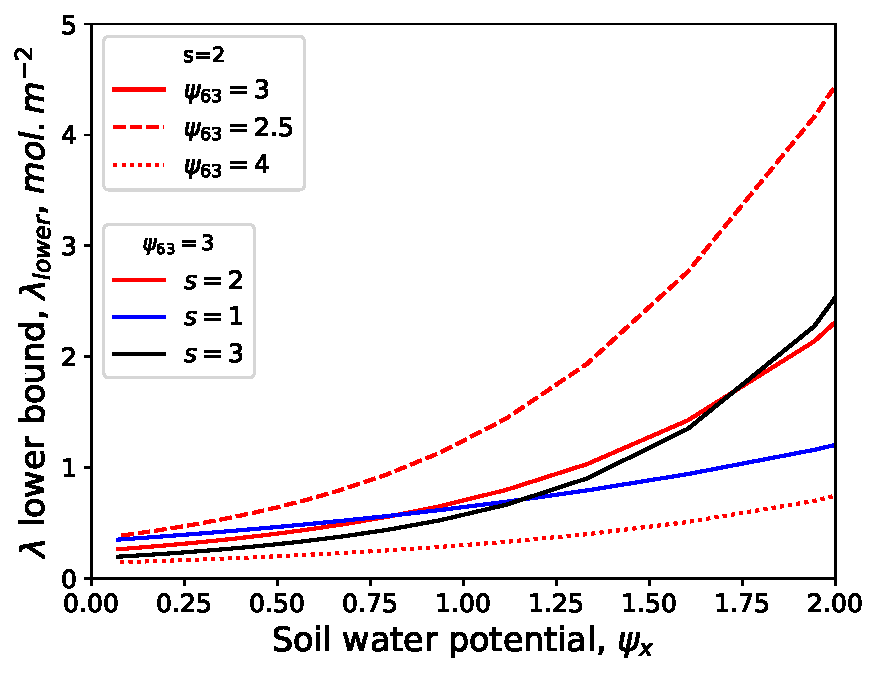
\includegraphics[scale=0.75]{Fig1.pdf}   
    \end{center}
    \caption{Diurnal trends of vapor pressure deficit (VPD), temperature ($T$), and photosynthetically active radiation (PAR). These are the averaged trends using measurements from the FLUXNET project at the Blodgett forest over 20 days starting from 5-29-2004 (the start of 4-months drought). These trends are repeated for the desired simulation duration.}
    \label{fig:environment}
\end{figure}

The model requires supplying environmental data acting as boundary conditions at the soil and leaf levels. These are the initial soil water content ($x_0$), vapor pressure deficit ($VPD$), incident leaf shortwave radiation ($R_l$), and temperature ($T$). We use the data provided by the FLUXNET project at the Blodgett forest. A drydown period starting on May 29, 2005 was chosen and the environmental variations over 20 days are averaged into one representative day. These conditions are then copied and tiled to however many days the optimization is running for. This allows isolating the plant hydraulic and strategy effects on stomatal behavior.

\section{Results}

\begin{table}[]
    \centering
    \begin{tabular}{c|c|c|c}
        Symbol & Property & Value & Unit \\
        \hline
        $g_{rl,max}$ & Maximum leaf area specific root-leaf hydraulic conductance & 10$^{-3}$ & mol m$^{-2}$ s$^{-1}$ MPa$^{-1}$ \\
        $g_{rl}$ & Leaf area specific root-leaf hydraulic conductance & varies & mol m$^{-2}$ s$^{-1}$ MPa$^{-1}$ \\
        $\psi_{63}$ & water potential at which $g_{rl} \approx 0.34 g_{rl,max}$ & varies & MPa \\
        $s$ & Shape parameter of the vulnerability curve & 2 &  \\
    \end{tabular}
    \caption{Plant properties used in the model unless stated in the particular simulation description, figure or table caption.}
    \label{tab:plant_props}
\end{table}
\begin{figure}[t]
    \begin{center}
        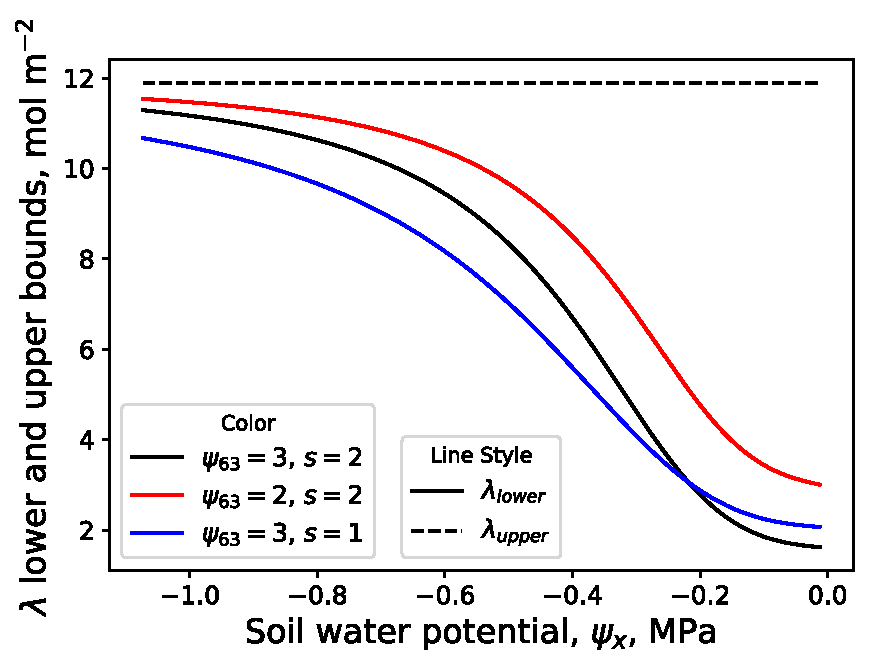
\includegraphics[width=10cm]{Fig2.pdf}
    \end{center}
    \caption{Hydraulic limits on $\lambda$. Vulnerability Curve (VC) alterations affect the lower limit ($\lambda_{lower}$). These alterations consist of changing the normalizing pressure $\psi_{63}$ and the slope $s$ of the VC (see equation \ref{eqn:root_leaf}). All of the shown curves are subject to environmental conditions at 12:00 on 5-29-2004 in Blodgett Forest (combination of vapor pressure deficit, temperature, and photosynthetically active radiation). The upper limit ($\lambda_{upper}$) is set at the point where $g_s=0$ because $g_s$ can never be negative.}
    \label{fig:lam_lower}
\end{figure}


As previously described, Soil-to-leaf plant hydraulics are prescribed through a Vulnerability Curve (VC). By setting an upper limit on $E$ and therefore $g_s$, the VC sets a lower limit on the value of the marginal use efficiency $\lambda$ (Figure \ref{fig:lam_lower}). Because of the inverse relation between $g_s$ and $\lambda$ (equation \ref{eqn:control}), an upper limit on $\lambda$ is set at $g_s=0$ because $g_s$ cannot be negative (equation \ref{eqn:control}). As the soil moisture decreases and the soil water potential gets more negative, the leaf is constrained to higher $\lambda$ while the upper limit maintains a constant value.

\begin{figure}
    \begin{center}
         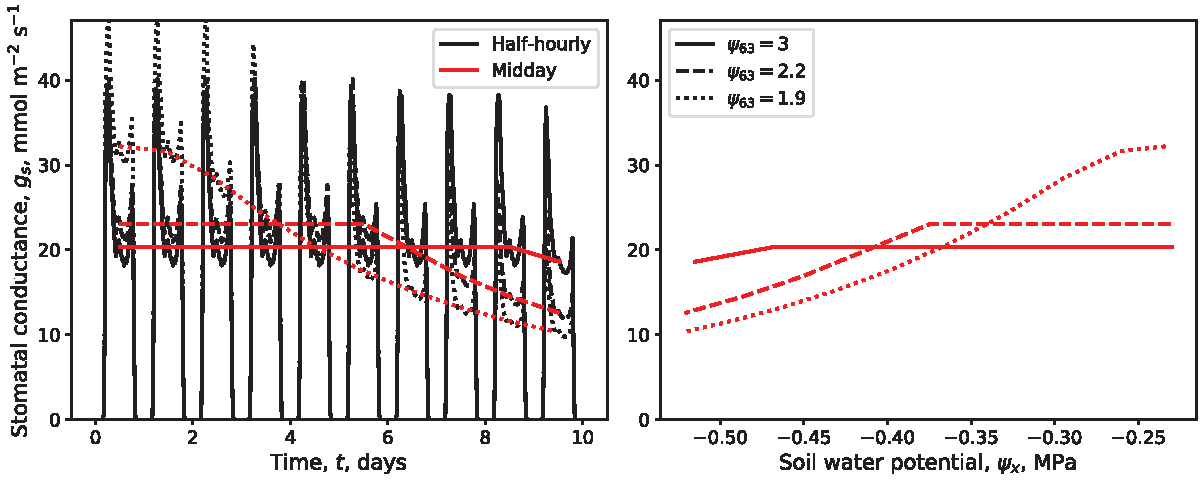
\includegraphics[scale=0.75]{Fig3.pdf}   
    \end{center}
    \caption{Half-hourly (black) and midday (red) trends of stomatal conductance ($g_s$) with a) time ($t$) and b) soil water potential ($\psi_x$). Trends are shown for a resistant plant ($\psi_{63} = 3$ MPa), a vulnerable plant ($\psi_{63} = 1.9$ MPa), and a midrange plant ($\psi_{63} = 2.2$ MPa). Other plant and soil parameters are listed in the appendix. The plant is Pinus radiata and soil is sandy loam.}
    \label{fig:resistant_vulnerable_gs}
\end{figure}

% The former of these two effects is shown in figure \ref{fig:lam_lower} where the lower bound of $\lambda$ ($\lambda_{lower}$) is plotted as a functions of soil water potential. This arises from the solution of equation \ref{eqn: dg} upon replacing A using equation \ref{eqn:A_noci}. The solution provides an inverse functional relationship between $g_l$ and $\lambda$. At every $\psi_x$, equation \ref{eqn: mass_cons} is maximized to obtain an upper bound on $g_l$ which translates into a lower bound on $\lambda$. Because the maximum possible transpiration rate $E$ decreases as $\psi_x$ increases, $\lambda_{lower}$ increases with $\psi_x$.

% The latter of these two effects is imposed through equation \ref{eqn: dlam}. In the simple case where no uncontrolled losses from the soil are present, $f=-E$ and therefore $\frac{d\lambda}{dt}=\lambda \frac{\partial E}{\partial x}$. Taking the partial derivative by $x$ of equation \ref{eqn: mass_cons} yields the following positively valued equation:
% \begin{equation}
%     \frac{\partial E}{\partial x} = g_p \Big(-\frac{\partial \psi_x}{\partial x}\Big) \Big[\frac{1}{2} \frac{s}{\psi_{63}} \Big(\frac{\psi_p}{\psi_{63}}\Big)^{s-1} (\psi_l-\psi_x) + 1\Big]
% \end{equation}


\section{Discussion}

The purpose of this work is to elucidate the connection of stomatal response to plant hydraulics and water-use strategy. Plant hydraulics was shown to set a lower limit for the marginal water-use efficiency ($\lambda$) whereas the upper limit is set by a ratio of atmospheric supply of carbon to atmospheric demand of water (figure \ref{fig:lam_lower}).

Connecting the concepts of isohydry and anisohydry to plant hydraulics represents a crucial next step toward improving stomatal response modelling. 

There is evidence for the evolutionary coordination between hydraulic traits and photosynthetic rate \citep{Scoffoni2016}. 

Fact that $psi_l$ only increases indicates irreversability in PLC.

\subsection{Figures}
Frontiers requires figures to be submitted individually, in the same order as they are referred to in the manuscript. Figures will then be automatically embedded at the bottom of the submitted manuscript. Kindly ensure that each table and figure is mentioned in the text and in numerical order. Figures must be of sufficient resolution for publication \href{http://home.frontiersin.org/about/author-guidelines#ResolutionRequirements}{see here for examples and minimum requirements}. Figures which are not according to the guidelines will cause substantial delay during the production process. Please see \href{http://home.frontiersin.org/about/author-guidelines#GeneralStyleGuidelinesforFigures}{here} for full figure guidelines. Cite figures with subfigures as figure \ref{fig:2}B.


\subsubsection{Permission to Reuse and Copyright}
Figures, tables, and images will be published under a Creative Commons CC-BY licence and permission must be obtained for use of copyrighted material from other sources (including re-published/adapted/modified/partial figures and images from the internet). It is the responsibility of the authors to acquire the licenses, to follow any citation instructions requested by third-party rights holders, and cover any supplementary charges.
%%Figures, tables, and images will be published under a Creative Commons CC-BY licence and permission must be obtained for use of copyrighted material from other sources (including re-published/adapted/modified/partial figures and images from the internet). It is the responsibility of the authors to acquire the licenses, to follow any citation instructions requested by third-party rights holders, and cover any supplementary charges.

\subsection{Tables}
Tables should be inserted at the end of the manuscript. Please build your table directly in LaTeX.Tables provided as jpeg/tiff files will not be accepted. Please note that very large tables (covering several pages) cannot be included in the final PDF for reasons of space. These tables will be published as \href{http://home.frontiersin.org/about/author-guidelines#SupplementaryMaterial}{Supplementary Material} on the online article page at the time of acceptance. The author will be notified during the typesetting of the final article if this is the case. 

\section{Nomenclature}

\subsection{Resource Identification Initiative}
To take part in the Resource Identification Initiative, please use the corresponding catalog number and RRID in your current manuscript. For more information about the project and for steps on how to search for an RRID, please click \href{http://www.frontiersin.org/files/pdf/letter_to_author.pdf}{here}.

\subsection{Life Science Identifiers}
Life Science Identifiers (LSIDs) for ZOOBANK registered names or nomenclatural acts should be listed in the manuscript before the keywords. For more information on LSIDs please see \href{http://www.frontiersin.org/about/AuthorGuidelines#InclusionofZoologicalNomenclature}{Inclusion of Zoological Nomenclature} section of the guidelines.


\section{Additional Requirements}

For additional requirements for specific article types and further information please refer to \href{http://www.frontiersin.org/about/AuthorGuidelines#AdditionalRequirements}{Author Guidelines}.

\section*{Conflict of Interest Statement}
%All financial, commercial or other relationships that might be perceived by the academic community as representing a potential conflict of interest must be disclosed. If no such relationship exists, authors will be asked to confirm the following statement: 

The authors declare that the research was conducted in the absence of any commercial or financial relationships that could be construed as a potential conflict of interest.

\section*{Author Contributions}

The Author Contributions section is mandatory for all articles, including articles by sole authors. If an appropriate statement is not provided on submission, a standard one will be inserted during the production process. The Author Contributions statement must describe the contributions of individual authors referred to by their initials and, in doing so, all authors agree to be accountable for the content of the work. Please see  \href{http://home.frontiersin.org/about/author-guidelines#AuthorandContributors}{here} for full authorship criteria.

\section*{Funding}
Details of all funding sources should be provided, including grant numbers if applicable. Please ensure to add all necessary funding information, as after publication this is no longer possible.

\section*{Acknowledgments}
This is a short text to acknowledge the contributions of specific colleagues, institutions, or agencies that aided the efforts of the authors.

\section*{Supplemental Data}
 \href{http://home.frontiersin.org/about/author-guidelines#SupplementaryMaterial}{Supplementary Material} should be uploaded separately on submission, if there are Supplementary Figures, please include the caption in the same file as the figure. LaTeX Supplementary Material templates can be found in the Frontiers LaTeX folder.

\section*{Data Availability Statement}
The datasets [GENERATED/ANALYZED] for this study can be found in the [NAME OF REPOSITORY] [LINK].
% Please see the availability of data guidelines for more information, at https://www.frontiersin.org/about/author-guidelines#AvailabilityofData

\bibliographystyle{frontiersinSCNS_ENG_HUMS} % for Science, Engineering and Humanities and Social Sciences articles, for Humanities and Social Sciences articles please include page numbers in the in-text citations
%\bibliographystyle{frontiersinHLTH&FPHY} % for Health, Physics and Mathematics articles
\bibliography{references}

%%% Make sure to upload the bib file along with the tex file and PDF
%%% Please see the test.bib file for some examples of references

\section*{Figure captions}

%%% Please be aware that for original research articles we only permit a combined number of 15 figures and tables, one figure with multiple subfigures will count as only one figure.
%%% Use this if adding the figures directly in the mansucript, if so, please remember to also upload the files when submitting your article
%%% There is no need for adding the file termination, as long as you indicate where the file is saved. In the examples below the files (logo1.eps and logos.eps) are in the Frontiers LaTeX folder
%%% If using *.tif files convert them to .jpg or .png
%%%  NB logo1.eps is required in the path in order to correctly compile front page header %%%

\begin{figure}[h!]
\begin{center}

\includegraphics[width=10cm]{logo1}% This is a *.eps file
\end{center}
\caption{ Enter the caption for your figure here.  Repeat as  necessary for each of your figures}\label{fig:1}
\end{figure}


\begin{figure}[h!]
\begin{center}
\includegraphics[width=15cm]{logos}
\end{center}
\caption{This is a figure with sub figures, \textbf{(A)} is one logo, \textbf{(B)} is a different logo.}\label{fig:2}
\end{figure}

%%% If you are submitting a figure with subfigures please combine these into one image file with part labels integrated.
%%% If you don't add the figures in the LaTeX files, please upload them when submitting the article.
%%% Frontiers will add the figures at the end of the provisional pdf automatically
%%% The use of LaTeX coding to draw Diagrams/Figures/Structures should be avoided. They should be external callouts including graphics.

\end{document}
